\documentclass[serif,mathserif]{beamer}
\usepackage{amsmath, amsfonts, epsfig, xspace}
\usepackage{algorithm,algorithmic}
\usepackage{pstricks,pst-node}
\usepackage{multimedia}
\usepackage[normal,tight,center]{subfigure}
\setlength{\subfigcapskip}{-.5em}
\usepackage{beamerthemesplit}
\usetheme{lankton-keynote}

\author[Tejaswi KC, Raj Krishnan]{Group 11 \\ Tejaswi KC \quad Raj Krishnan \\ 140010020 \quad 140010007}

\title[PyAlpha\hspace{2em}\insertframenumber/\inserttotalframenumber]{PyAlpha: Final Report}

\institute{Indian Institute of Technology, Bombay}

\begin{document}

    \maketitle

    \begin{frame}

        \frametitle{Tasks}

        \begin{itemize}
            \item Build a python module to handle the purchase and sale of stocks
                  as per current prices on the share markets
            \item Build a module to compute the quality of various alphas
                  (weights for various stocks)
            \item Hosted at \url{https://github.com/raj-krishnan/PyAlpha}
        \end{itemize}

    \end{frame}

    \begin{frame}

        \frametitle{Tests}
        
        \textbf{Testsuite:}
        \begin{figure}
            \centering
            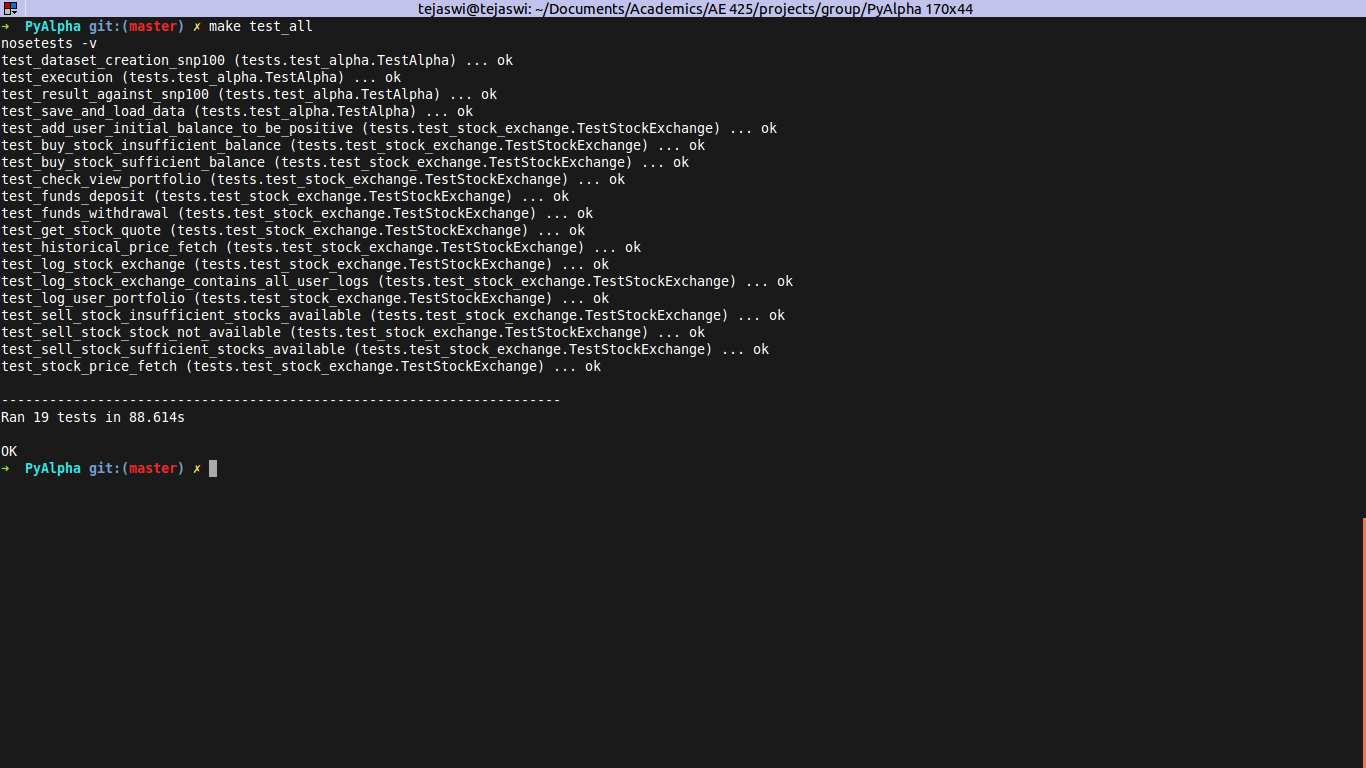
\includegraphics[width = \linewidth]{testsuite.png}
        \end{figure}

    \end{frame}
    
    \begin{frame}{Coverage}

        \textbf{Coverage:}
        \begin{figure}
            \centering
            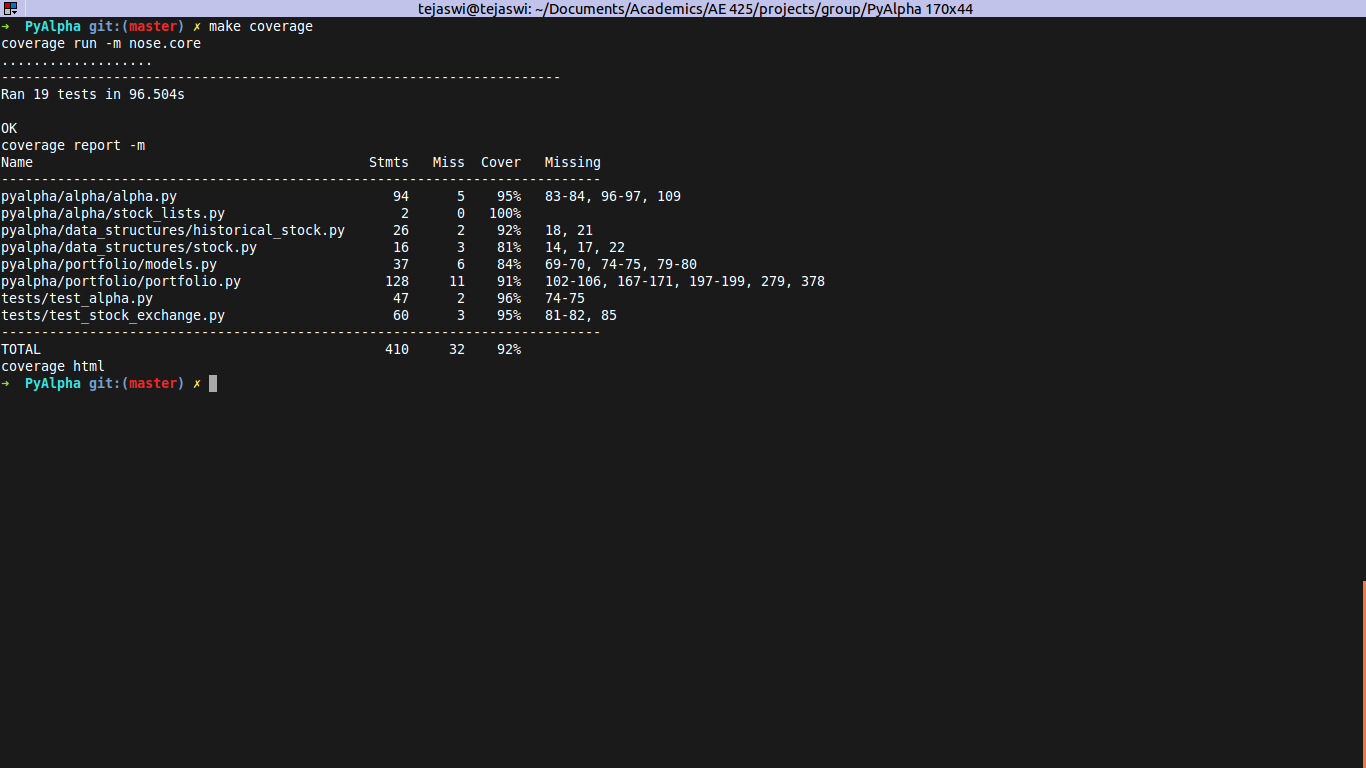
\includegraphics[width = \linewidth]{coverage.png}
        \end{figure}
        
    \end{frame}
    
    \begin{frame}{Automation}
    
        \begin{itemize}
            \item Continuous Integration using \href{https://travis-ci.org/raj-krishnan/PyAlpha}{Travis}
            \item Coverage Testing using \href{https://coveralls.io/github/raj-krishnan/PyAlpha}{Coveralls}
        \end{itemize}
        
    \end{frame}
    
    \begin{frame}

        \frametitle{Installation using git}

        \begin{itemize}
            \item git clone https://github.com/raj-krishnan/PyAlpha.git
            \item cd PyAlpha
            \item pip install -r requirements.txt
            \item python setup.py install
        \end{itemize}

    \end{frame}
    
    \begin{frame}{Docs}
    
        \begin{itemize}
            \item Documentation hosted at \url{http://pyalpha.readthedocs.io/}
        \end{itemize}
        
    \end{frame}
    
    \begin{frame}{Code cleanliness}
        
        \begin{itemize}
            \item Using PEP8
        \end{itemize}
        
    \end{frame}
    
    \begin{frame}{Git commit graphs}
    
        % \begin{itemize}
        %     \item 
        % \end{itemize}
        
    \end{frame}

    \begin{frame}

        \frametitle{Dependencies}

        \begin{itemize}
            \item pandas
            \item peewee
            \item ystockquote
        \end{itemize}

    \end{frame}

    \begin{frame}

        \frametitle{Portfolio Handling Demo}

        \begin{figure}[h]
            \centering
            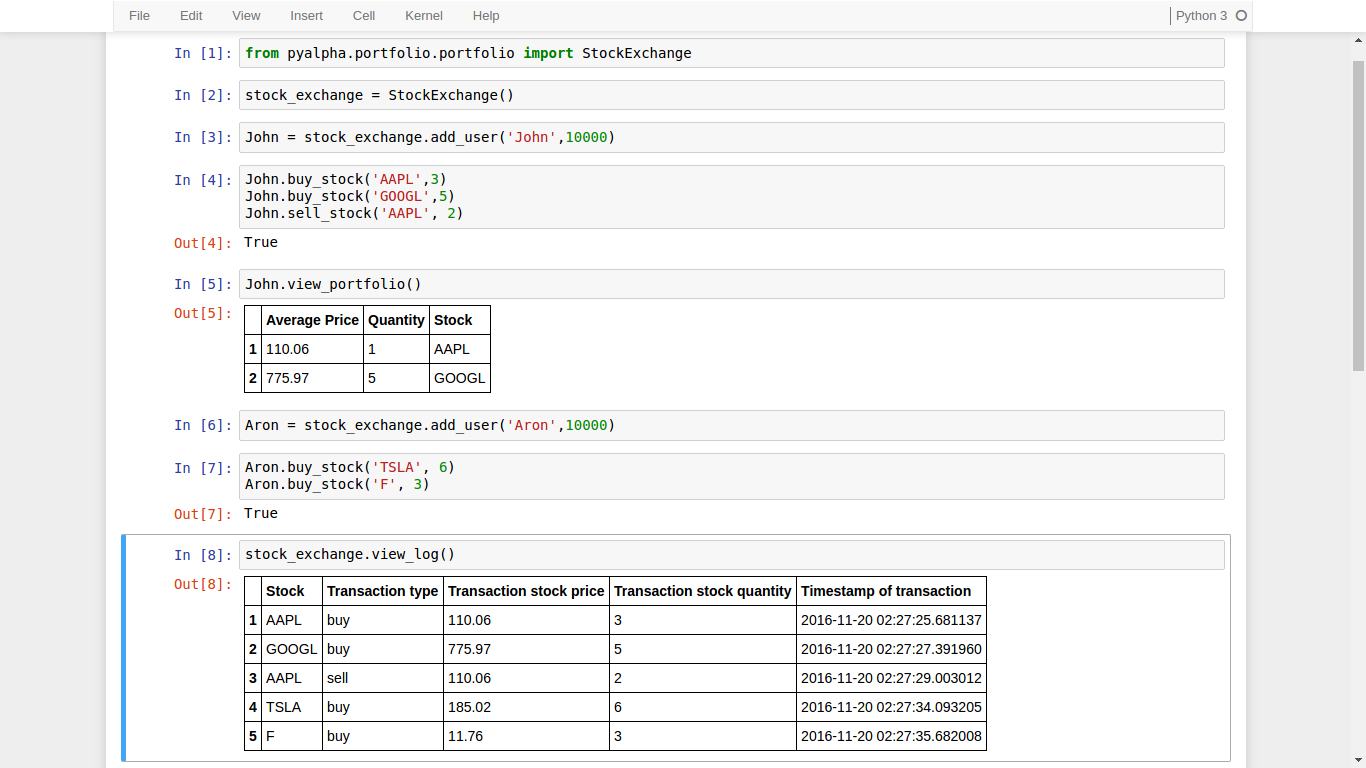
\includegraphics[width=\linewidth]{portfolio.png}
        \end{figure}

    \end{frame}

    \begin{frame}
        \centering \huge{Thank You!}
    \end{frame}

\end{document}
